Identifying the forces driving change in natural systems is a major goal in ecology. 
Because experiments are often impractical and come at the cost of generalizability, a common approach is to fit mechanistic models to observations. 
Testing hypotheses through mechanistic models has a particularly strong tradition in infectious disease ecology \cite{KeelingRohani, AndersonMay, Kermack1927, Ross1910}.
Models that incorporate both rainfall and host immunity, for example, better explain patterns of malaria than models with only rainfall \cite{Laneri2010}; models with school terms fit the historic periodicity of measles in England and Wales \cite{Finkenstadt2000, Fine1982}.
The ability of fitted mechanistic models to predict observations outside the training data strongly suggests that biological insight can be gained. There is nonetheless a pervasive risk that predictive variables merely correlate with the true, hidden variables, or that the model's functional relationships create spurious resemblances to the true dynamics. 
This structural uncertainty in the models themselves limits inference \cite{BurnhamAnderson, He2009, Yodzis1988, Wood1999, Grad2012}. 

An alternative approach to inferring causality is to examine the time series of potentially interacting variables without invoking a model. 
These methods face a similar challenge: they must distinguish correlated independent variables sharing a mutual driver from correlations arising from direct or indirect interactions. 
Many of these methods, including Granger causality~\cite{Granger1969} and other related methods~\cite{Schumacher2015,Mooij2014,Stegle2010}, infer interactions in terms of information flow in a probabilistic framework and cannot detect bidirectional causality.
A recent suite of methods based on dynamical systems theory proposes to infer interactions, both unidirectional and bidirectional, in systems that are nonlinear, noisy, and potentially high-dimensional \cite{Sugihara2012, Ye2015, Clark2015}.
The basic idea is that if $X$ drives $Y$, information about $X$ is embedded in the time series of $Y$.
Examining the relationships between delay-embeddings of the time series of $X$ and $Y$ can reveal whether $X$ drives $Y$, $Y$ drives $X$, both, or neither.
These approaches, which we refer to collectively as convergent cross-mapping (CCM), have been offered as general tools to analyze causation in nonlinear dynamical systems \cite{Sugihara2012, Ye2015, Clark2015}.

\begin{figure}
    \begin{center}
        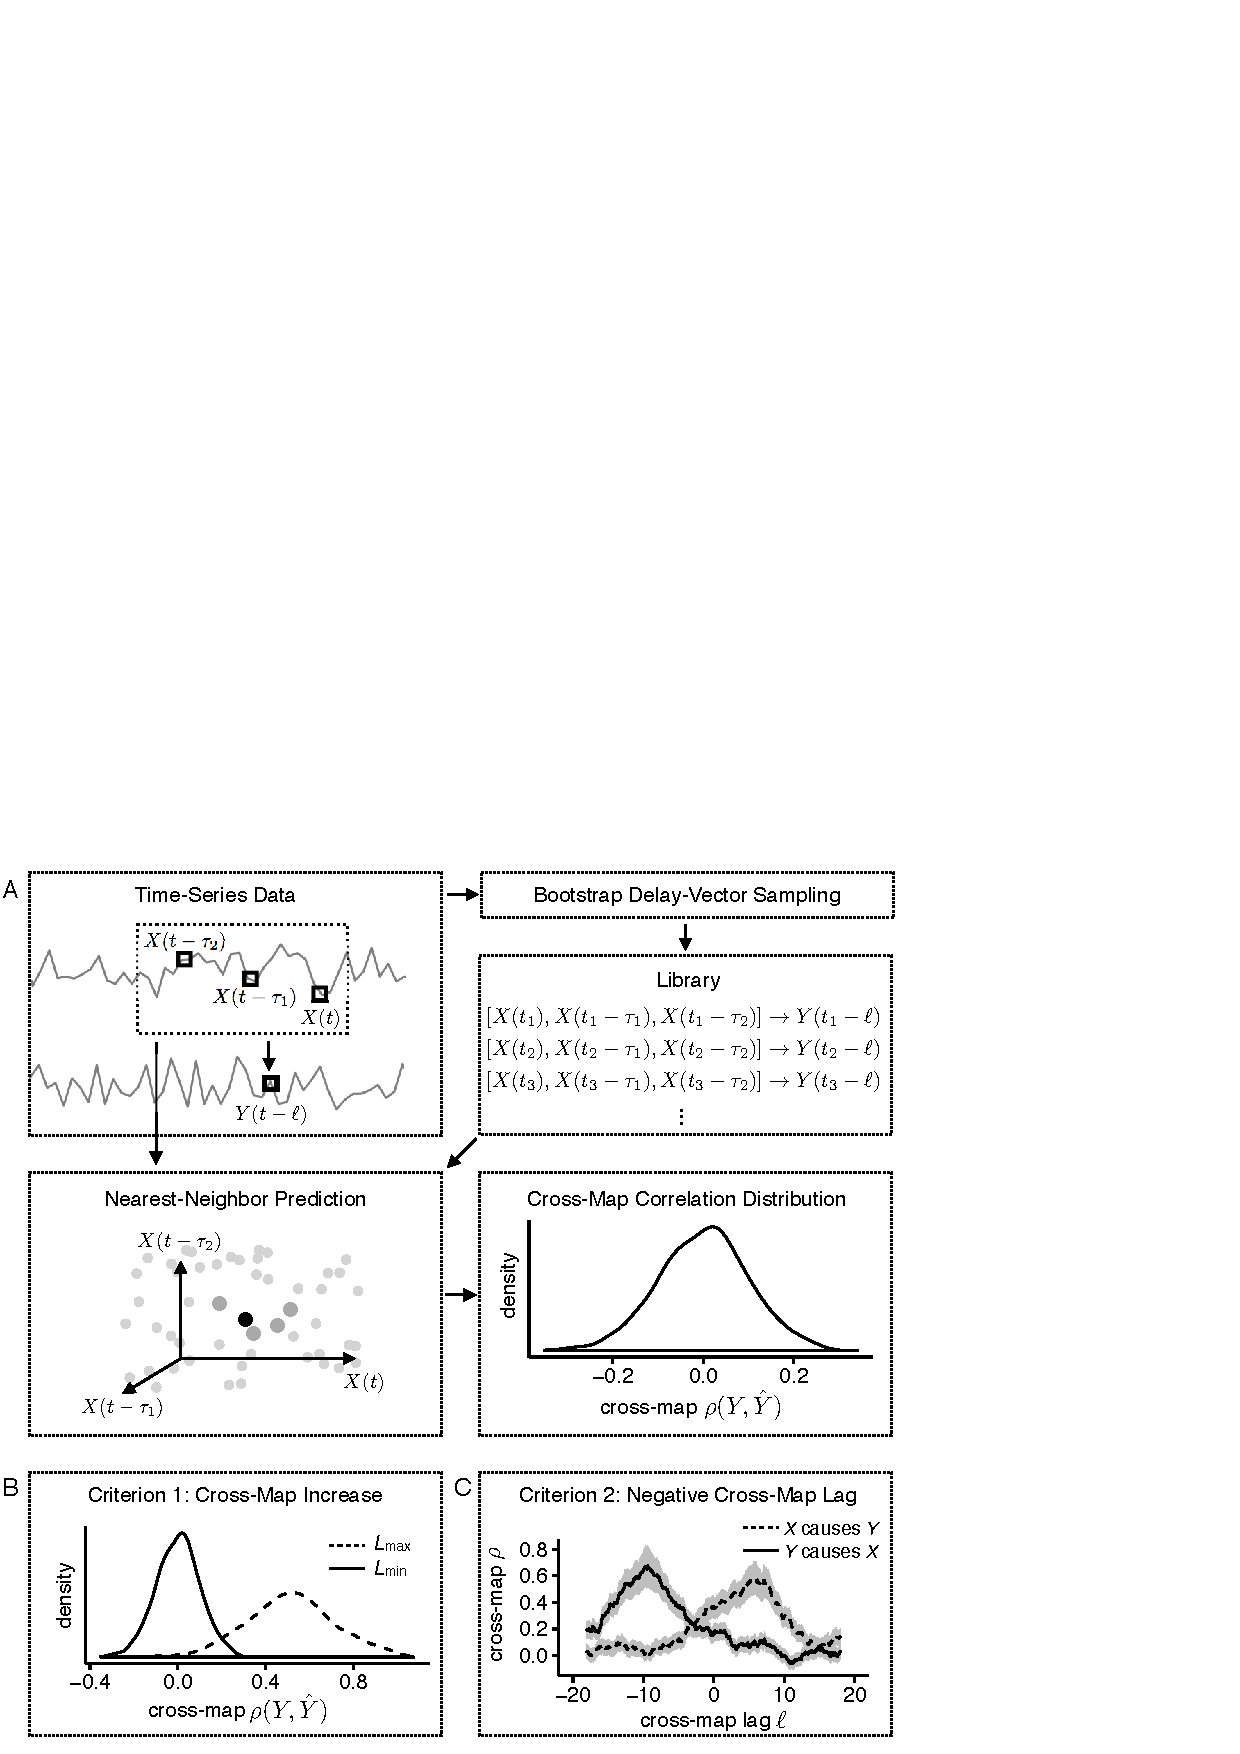
\includegraphics[width=6in]{dataflow/out/fig_conceptual/fig_conceptual.pdf}
    \end{center}
    \caption{\textbf{Summary of criteria for detecting causality}. (A) Schematic of cross-map algorithm for testing $Y \rightarrow X$. Delay vectors in $X$, mapped to values in $Y$ with lag $\ell$, are bootstrap-sampled to construct a prediction library. For each delay vector in $X$, reconstructed values $\hat{Y}$ are calculated from a distance-weighted sum of $Y$ values from nearest neighbors in the library. Many sampled libraries yield a distribution of cross-map correlations between actual $Y$ and reconstructed $\hat{Y}$. (B) Criterion 1 (cross-map increase). Bootstrap distributions of cross-map correlation are calculated at minimum and maximum library sizes with $\ell = 0$; causality is inferred if the correlation at $L_{\max}$ is significantly greater than the correlation at $L_{\min}$. (C) Criterion 2 (negative cross-map lag). Cross-map correlations are calculated across different values of $\ell$. Causality is inferred if the highest cross-map correlation for negative $\ell$ is positive and significantly greater than the highest value for nonnegative $\ell$. \label{fig:conceptual}}
\end{figure}

The mathematical foundations of CCM, and therefore its assumptions, lie in deterministic nonlinear systems theory.
After sufficient time, the states of a deterministic dynamical system reach an attractor, which may be a point equilibrium, a limit cycle, or a higher-dimensional chaotic attractor.
By Takens' theorem, a one-dimensional time series $X(t)$ from the system can be mapped perfectly to the attractor in the full state space in the system by constructing a delay embedding, in which states of the full system are mapped to delay vectors, $\bx(t) = \{X(t), X(t - \tau_1), X(t - \tau_2), \ldots, X(t - \tau_{E-1} \}$, for \emph{delays} $\tau_i$ and an \emph{embedding dimension} $E$, which must be at least as large as the dimensionality of the attractor~\cite{Takens1981}.
This mapping provides the basis for causal inference under CCM: if $Y$ drives (causes) $X$, then a newly observed $\bx(t)$ can perfectly reconstruct the corresponding $\hY(t)$ from past observations of the mapping $\bx(t) \rightarrow Y(t)$ (Fig.~\ref{fig:conceptual}A).
As the number of observed delay vectors $\bx(t)$ increases, the reconstruction converges to small error, as observed points on the reconstructed attractor become close together~\cite{Sugihara2012}.

With finite, noisy real data, the reconstruction is necessarily imperfect, and two operational criteria have been used to detect causality.
The first criterion (Fig.~\ref{fig:conceptual}B) is based simply on this improvement in reconstruction quality with the number of observations.
This approach is known to produce false positives in the case of strongly driven variables, where the system becomes synchronized to the driver \cite{Sugihara2012, Kocarev1996}.
This failure is logically consistent with the theory: the theory implies that, with perfect data, causal drivers will produce good reconstructions, but not that non-causal drivers will not produce good reconstructions.
The second criterion (Fig.~\ref{fig:conceptual}C) tries to correct this problem by additionally considering the directionality of information flow in time~\cite{Ye2015}.
If one variable drives another, the best predictions of current states of the driven variable should come from past, not current or future, states of the driver.

Many ecological systems undergo synchronized diurnal or annual fluctuations and thus raise doubts about the first criterion.
Transient dynamics, demographic and environmental noise, and observation error---all ubiquitous in nature---raise general concerns, since they violate the theory's assumption that variables are perfectly observed in a deterministic system.
Variations of CCM have nonetheless been applied to such systems to test hypotheses about who interacts with whom \cite{Ye2015, Sugihara2012, Tajima2015, Tsonis2015, Clark2015}.

We investigated whether the frequently periodic, noisy, and transient dynamics of ecological systems are a current obstacle to causal inference based on state-space reconstruction.
These factors have been addressed to varying degrees in different contexts \cite{Sugihara2012, Ye2015, Clark2015} but not systematically.
Specifically, we examined whether the two criteria for causal inference are robust to inevitable uncertainties about the dynamics underlying the data.
With little prior knowledge of a system's complexity, including the influences of transient dynamics and noise, can we reach statistically rigorous conclusions about who interacts with whom?
Infectious diseases provide a useful test case because their dynamics have been extensively studied, long time series are available, and pathogens display diverse immune-mediated interactions \cite{Cobey2014}.  
Their dynamics are also influenced by seasonal variation in transmission rates, host population structure, and pathogen evolution.  
The ability to test directly for the presence of interactions would save considerable effort over fitting semi-mechanistic models that incorporate these complexities.
We find that although CCM appears to work beautifully in some instances, it does not in others.
Noise and transient dynamics contribute to poor outcomes, as do statistical ambiguities in the methodology itself.
We propose that except in extreme circumstances, the current method cannot reliably reveal causality in natural systems.
